\subsection{Hebel \hfill IP}
\begin{footnotesize}
    \begin{center}
        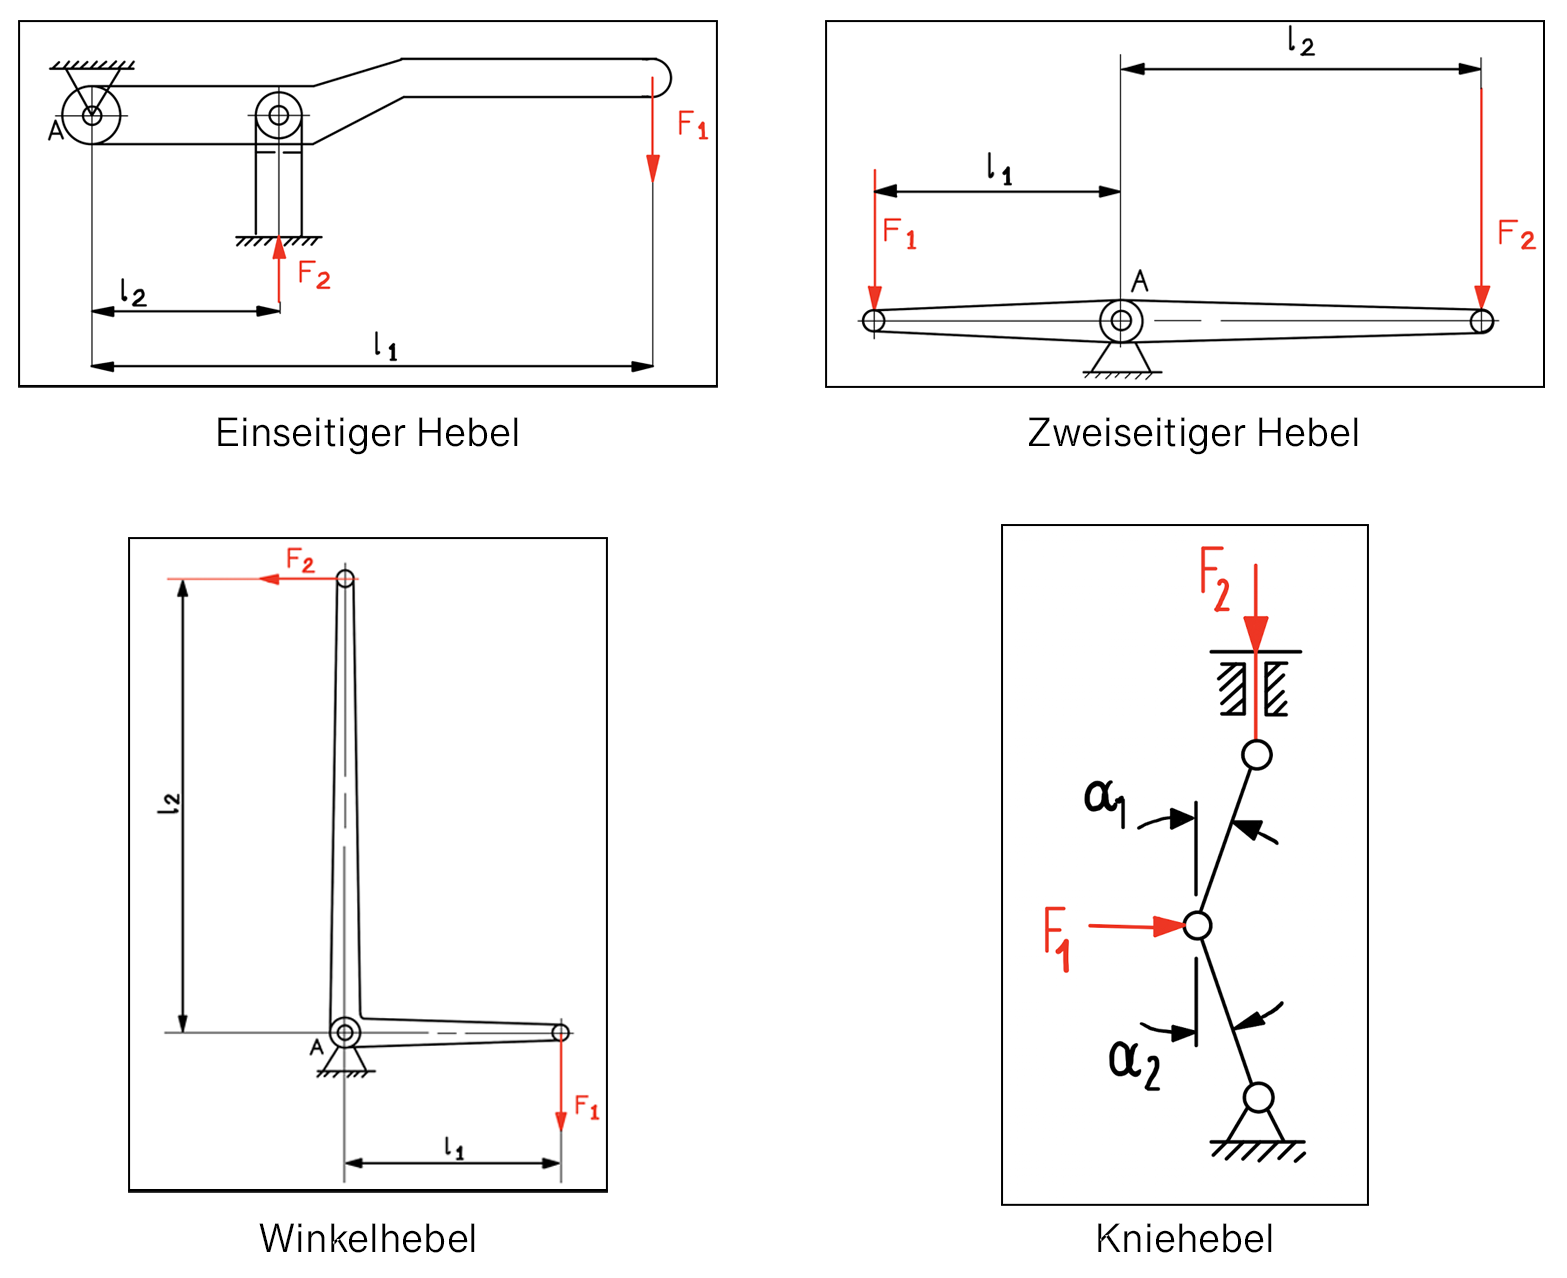
\includegraphics[width = 0.8\linewidth]{MAEIP_Hebel}
        \includegraphics[width = 0.5\linewidth]{MAEIP_Serienhebel}
    \end{center}
\cbreak

    \begin{empheq}[box=\fbox]{align*}
        \textbf{Allgemein: }F_2 &= \frac{l_1}{l_2}\cdot F_1
        \\\textbf{Kniehebel: }F_2 &= \frac{F_1}{tan(\alpha_1) + tan(\alpha_2)} 
        \\\textbf{Serienschaltung: }F_3 &= \frac{l_1}{l_2} \cdot \frac{l_3}{l_4} \cdot F_1
    \end{empheq}
\end{footnotesize}